\chapter{Artefact Design} \label{chap:artefact-design}
\section{Development decisions}
\subsection{Software development methodology}
In the software development life cycle there are various stages: requirements gathering, analysis, design,
development, testing, deployment and maintenance.\\
The Agile software development methodology will be utilised in this project; and this project will be separated
into various iterations of design, development, and testing. This will allow for a more flexible approach to
the task and the ability to make changes as the project progresses without requiring additional time and effort
to fully test and deploy an inaccurate or unsuitable artefact.
\begin{figure}
    \centering
    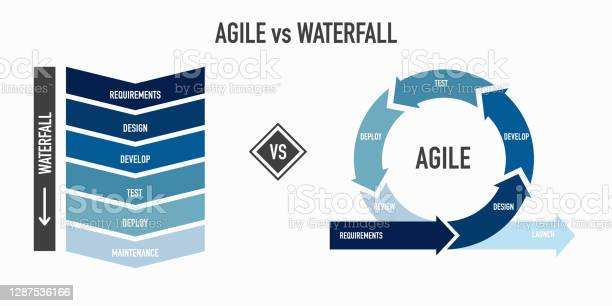
\includegraphics[width=\columnwidth]{figures/development_methodologies.jpg}
    \caption{A comparison of the Agile and Waterfall methodologies (source: iStock, iam2mai)
    (replace as there is a copyright)}
    \label{fig:development_methodologies}
\end{figure}
\FloatBarrier

\subsection{Software languages and libraries}
\subsubsection{Programming Language}
Python has been chosen to be used in this project as it is ubiquitous for artificial intelligence related
tasks. There are many resources readily available for Python with regards to its usage on artificial
intelligence models and neural networks. There are various Python libraries for machine learning applications
such as Tensorflow, an `end-to-end open source machine learning platform' created by Google as well as
PyTorch, ` open source machine learning framework' created by Facebook's AI Research Lab.

\subsubsection{Python libraries for machine learning}
As mentioned in the previous section there are various machine learning libraries for Python. Currently, the
most popular is Tensorflow and has the most resources available.
However, the usage of PyTorch has accelerated over the past years and is quickly becoming the preferred
library as it is considered to be more `pythonic' and often quicker to train neural networks.

Tensorflow will be used in the project due to its current ubiquity in this task, especially surrounding
its applications for financial forecasting. However, PyTorch may be chosen for future iterations if
the performance of Tensorflow is found to be insufficient and the performance of PyTorch is found to be
greater.

\section{Input features chosen and data collection}
The input features chosen are an amalgamation primarily based on those found in the literature review.
From the literature review, the input features have been classified into four categories:
\begin{itemize}
    \item Stock market index
    \item Money availability
    \item Alternative portfolio allocations
    \item Sentiment
\end{itemize}

From this, the following sources for input features have been chosen; the reasoning are explained and the
sources for used in the data collection process are also present within this list.
\begin{itemize}
    \item Stock market index
    \begin{itemize}
        \item Closing price\\
        \textbf{Reasoning:} It is believed that a sequence of closing price returns
        can be utilised to predict a future closing price\\
        \textbf{Source:} Yahoo Finance - SPY Historical Data:\\
        https://uk.finance.yahoo.com/quote/SPY/history
        \item Volume\\
        \textbf{Reasoning:} It is believed that the amount of stock traded can indicate
        confidence in that stock market index and potentially future price movements\\
        \textbf{Source:} Yahoo Finance - SPY Historical Data:\\
        https://uk.finance.yahoo.com/quote/SPY/history
        \item Volatility (based on VIX)\\
        \textbf{Reasoning:} It is believed that the volatility in the stock market can potentially
        indicate future price movements\\
        \textbf{Source:} Yahoo Finance - VIX Historical Data:\\
        https://uk.finance.yahoo.com/quote/\%5EVIX/history
    \end{itemize}
    \item Money availability
    \begin{itemize}
        \item M1 Money Supply\\
        \textbf{Reasoning:} It is believed that a change in total money supply circulation can affect
        the amount of money allocated to the stock market, such as with measures related to quantitative
        easing to affect stock returns\\
        \textbf{Source:} Federal Reserve Economic Data - M1 Money Supply:\\
        https://fred.stlouisfed.org/series/WM1NS
        \item GDP\\
        \textbf{Reasoning:} It is believed that the GDP can affect the money available to market
        participants and thus impact stock returns\\
        \textbf{Source:} Federal Reserve Economic Data - GDP:\\
        https://fred.stlouisfed.org/series/GDP
    \end{itemize}
    \item Alternative portfolio allocations
    \begin{itemize}
        \item Treasury Yields
        \begin{itemize}
            \item 1Mo
            \item 3Mo
            \item 1Yr
            \item 2Yr
            \item 5Yr
            \item 10Yr
            \item 20Yr
            \item 30Yr
        \end{itemize}
        \textbf{Reasoning:} It is believed that the market participants often allocate their funds
        to treasury bonds / bills / notes for a guaranteed return compared to risk in the stock market.
        A change to yields may affect the money allocated in the stock market and thus affect the
        return of the stock market index.\\
        \textbf{Source:} US Dept. of the Treasury - Treasury Par Yield Curve Rates:\\
        % \seqsplit{https://home.treasury.gov/resource-center/data-chart-center/interest-rates/TextView?type=daily_treasury_yield_curve}
        \item Effective Federal Funds Rate\\
        \textbf{Reasoning:} EFFR is the interest rate banks charge one another for overnight loans, a change in 
        EFFR may affect the loans banks make / take and thus affect the money the banks have available to allocate
        in the stock market; this may affect the return of the stock market index.\\
        \textbf{Source:} Federal Reserve Economic Data - EFFR:\\
        https://fred.stlouisfed.org/series/EFFR
        \item Repurchase / Reverse Repurchase Agreements\\
        \textbf{Reasoning:} A change in utilisation of repurchase agreements may indicate if banks expect
        a greater return elsewhere and how banks are allocating money. This may have an impact on the 
        return of the stock market index\\
        \textbf{Source:} New York Fed - Repo:\\
        https://www.newyorkfed.org/markets/desk-operations/repo
        \item Gold\\
        \textbf{Reasoning:} It is believed that a change in the prices of commodities such as gold may be
        an indicator of portfolio allocation changes; thus affecting the return of the stock market index\\
        \textbf{Source:} London Bullion Market Association - Precious Metal Prices:\\
        https://www.lbma.org.uk/prices-and-data/precious-metal-prices\#/table
        \item Foreign Currency
        \begin{itemize}
            \item USD-GBP\\
            \textbf{Source:} Federal Reserve Economic Data - GBP:\\
            https://fred.stlouisfed.org/series/DEXUSUK
            \item USD-EUR\\
            \textbf{Source:} Federal Reserve Economic Data - EUR:\\
            https://fred.stlouisfed.org/series/DEXUSEU
            \item USD-JPY\\
            \textbf{Source:} Federal Reserve Economic Data - GBP:\\
            https://fred.stlouisfed.org/series/DEXJPUS
        \end{itemize}
        \textbf{Reasoning:} It is believed that the currency exchange rates may be an indicator of confidence
        of the country of the currency, thus a change in currency rate may result in a change of portfolio
        allocations of participants in that country's stock market.        
    \end{itemize}
    \item Sentiment
    \begin{itemize}
        \item Put-to-Call Ratio\\
        \textbf{Reasoning:} It is believed that the market participants may use the options market
        to speculate on future returns of the stock market. The put to call ratio indicates the sentiment
        of the market participants and may have an affect on the return of the stock market index.\\
        \textbf{Source:} AlphaAlerts: Historical Equity Put/Call Ratio\\
        https://www.alphalerts.com/live-historical-equity-pcr/
        \item Employment Rate\\
        \textbf{Reasoning:} It is believed that market participants may react to changes of employment
        rate in making investment decisions. A change in nationwide employment may cause market participants
        to change their portfolio allocations due to lesser confidence in ability for companies in the country
        to produce and sell; thus potentially affect the return of the stock market index.\\
        \textbf{Source:} Federal Reserve Economic Data - Employment Rate:\\
        https://fred.stlouisfed.org/series/LREM64TTUSM156S
        \item Inflation Rate\\
        \textbf{Reasoning:} It is believed that a change in inflation rate can cause market participants
        to change their portfolio allocations and thus affect the return of the stock market\\
        \textbf{Source:} US Bureau of Labor Statistics - Inflation:\\
        https://www.bls.gov/data/\#prices
    \end{itemize}
\end{itemize}


\section{Assumptions made}
The primary assumptions are surrounding the trading days; whilst this varies per month / year, it is assumed
that 1 week is equivalent to 5 trading days, 1 month is equivalent to 21 trading days, 1 quarter (3 months)
is equivalent to 63 trading days, 1 half is equivalent to 126 trading days, and 1 year is equivalent to 252
trading days.
\section{Data normalisation}

\section{Iteration 1}
\subsection{Artificial intelligence model used}
\subsection{Sequence length used}
\subsection{Input features}
\subsection{Accuracy of iteration 1}
\subsection{Limitations of iteration 1}